\chapter{Plataforma de recomendaciones}
\label{chap:software}
\graphicspath{{/Users/brunomedina/Dropbox/Tesis-Egobets/egobets-notas/resources/diagramas/}}

Egobets.com proporciona al cliente los servicios de asesoría de apuestas personalizada a través de un portal Web usable, práctico y profesional. En este capítulo se presenta el sistema desarrollado con los fundamentos teóricos descritos en los capítulos anteriores, una verdadera aplicación computacional de las matemáticas

% Se describen las cuatro piezas de software desarrolladas que conforman en su totalidad el sistema de Egobets. Las tres primeras permiten al usuario adminstrativo echar a andar toda la maquinaria. Y la última pieza, conocida como e
% A todo este conjunto de herramientas y programas que el usuario necesita para esta tarea se le conocerá como \emph{Back Office}.




\section{Diseño y arquitectura}
\label{sec:design}
Egobets.com es un sistema con arquitectura cliente-servidor montado sobre una máquina virtual con sistema operativo Ubuntu Linux en la nube de ``Amazon Web Services (AWS)''. En esta sección se presentan los diagramas que describen la arquitectura del sistema, se muestran las ventajas de utilizar el cómputo en la nube, se presentan las tecnologías más relevantes involucradas en el sistema y también se expone el patrón de diseño \textit{Modelo Vista Controlador} junto con su respectiva representación gráfica de base de datos.
\subsection{Ventajas de correr Egobets en la nube}
\begin{figure}[!htb]\centering
   \begin {minipage}{1\textwidth}
     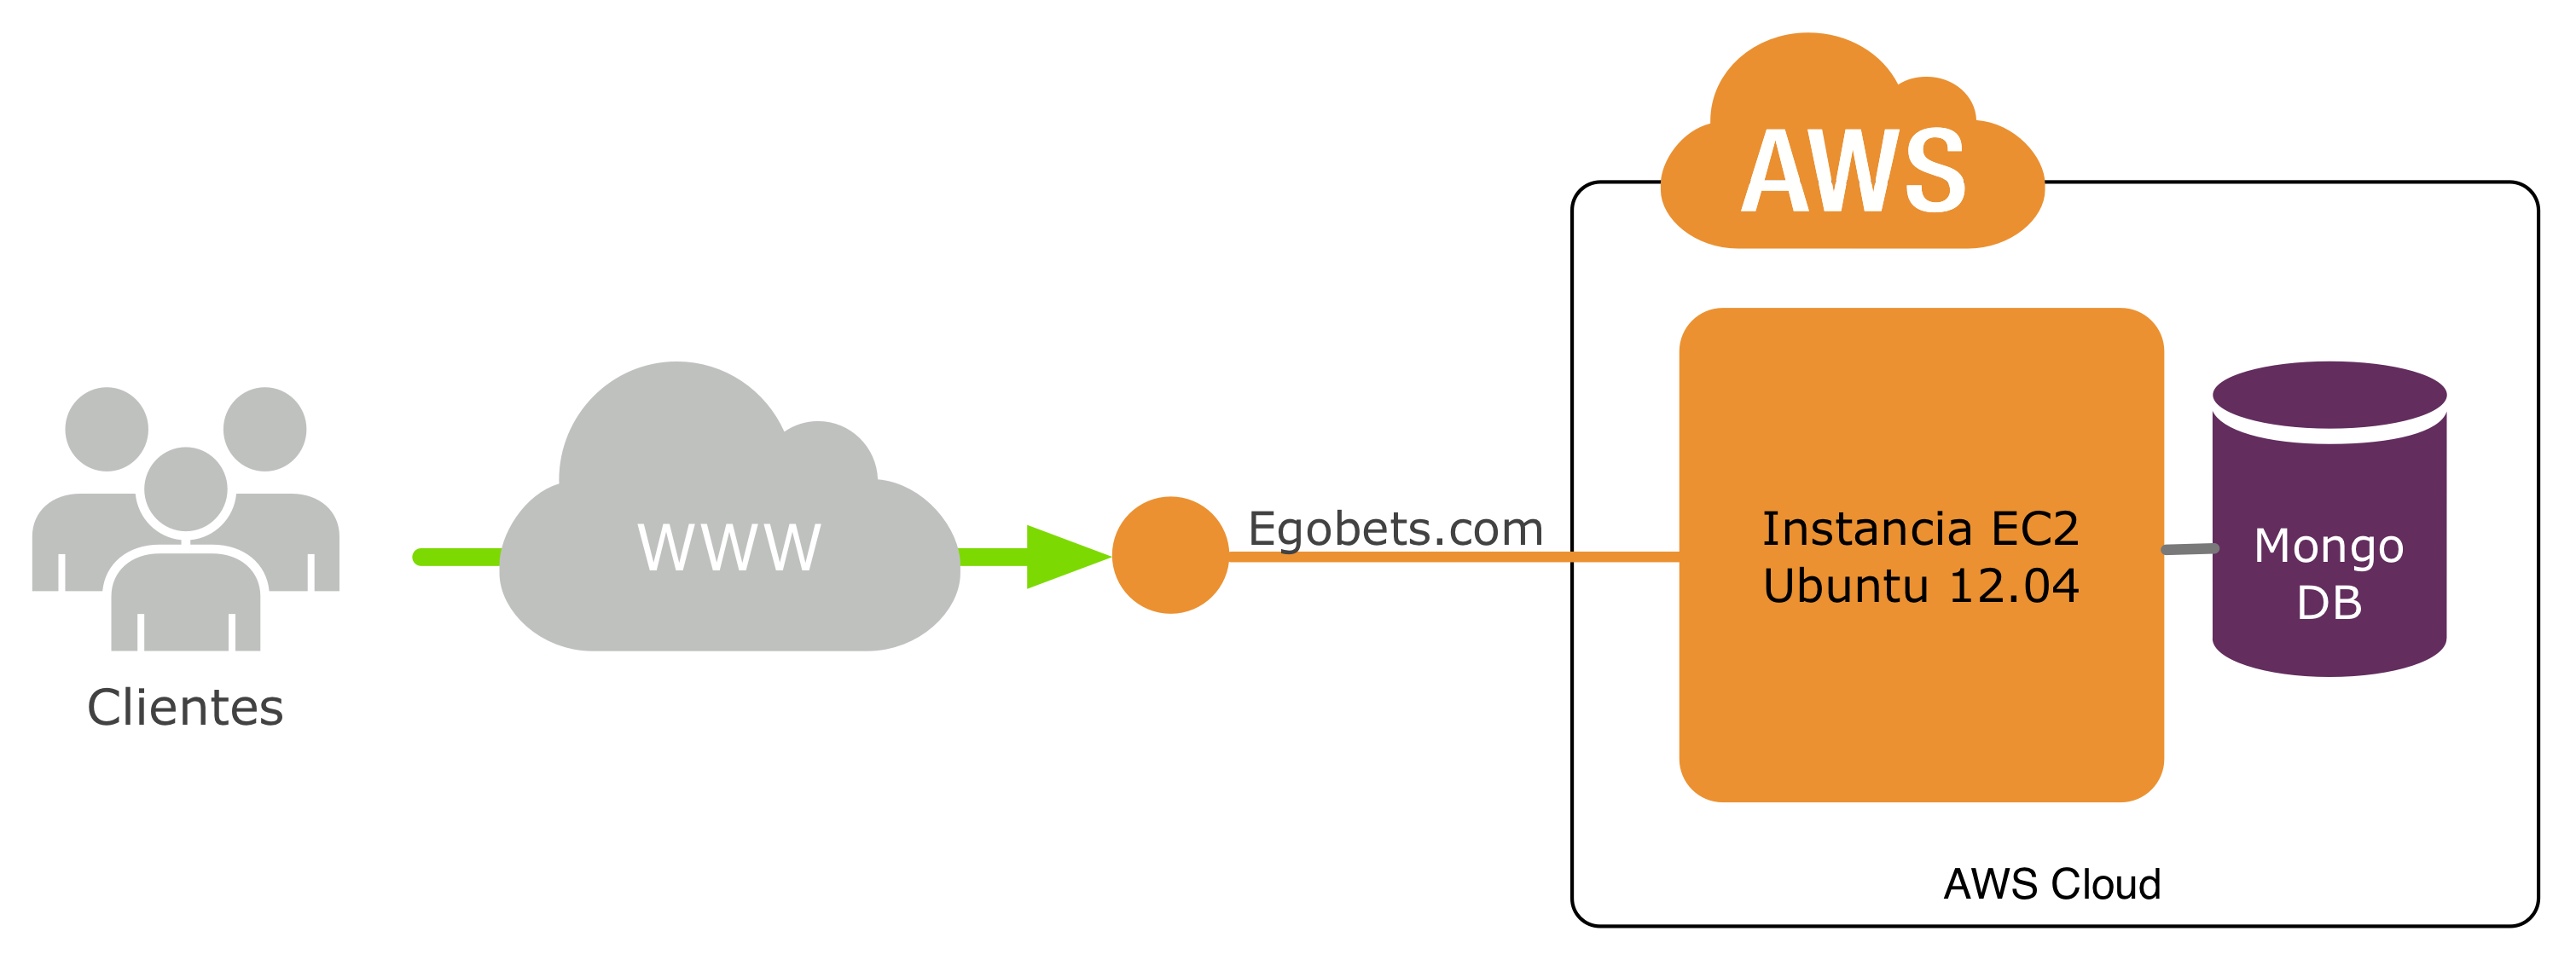
\includegraphics[width=\linewidth]{diagrama-portal-publico}
     \caption{Arquitectura Cliente Servidor sobre Nube de AWS}\label{Fig:diagrama-portal-publico}
   \end{minipage}
\end{figure}

El sistema usa la nube de AWS para ofrecer sus servicio a los usuarios (Véase la imagen~\ref{Fig:diagrama-portal-publico}), más aún se puede decir que el software corre en un esquema tipo ``SaaS''\footnote{Software as a Service. ``Es el más conocido de los niveles de cómputo en la nube. El SaaS es un modelo de distribución de software que proporciona a los clientes el acceso a éste a través de la red (generalmente Internet). De esta forma, ellos no tienen que preocuparse de la configuración, implementación o mantenimiento de las aplicaciones, ya que todas estas labores se vuelven responsabilidad del proveedor. Las aplicaciones distribuidas a través de un modelo de Software como Servicio pueden llegar a cualquier empresa sin importar su tamaño o ubicación geográfica.'' \cite{godinez2010nube}.}, esto implica que el usuario simplemente ingresa a su cuenta en un navegador de internet y puede ver las asesorías para sus apuestas.
Del artículo ``Cómputo en Nube: Ventajas y Desventajas'' de Martínez y Gutiérrez \cite{godinez2010nube}  se retoman las siguientes ventajas de este paradigma:
\begin{itemize}
	\item \textbf{Costos.} Podría ser la ventaja más atractiva que presenta el cómputo en la nube, y si no lo es, al menos es la más evidente de todas las que ofrece esta tecnología. Al dejar la responsabilidad de la implementación de la infraestructura al proveedor, el cliente no tiene que preocuparse por comprar equipos de cómputo, capacitar personal para la configuración y mantenimiento de éstos, y en algunos casos, por el desarrollo del software. Además el usuario de estos servicios únicamente paga por los recursos que utiliza, permitiéndole diseñar un plan de pago normalmente a partir del tiempo en que éste se utiliza (memoria, procesamiento, almacenamiento). Para Egobets, esta cualidad es vital, ya que en el comienzo después de haber implantado el software, la cantidad de usuarios es mínima y los ingresos también. Conforme crece la bolsa de clientes también irá creciendo la potencia de la infraestructura.

	\item \textbf{Competitividad.} Al no tener que adquirir equipos costosos, las pequeñas empresas pueden tener acceso a las más nuevas tecnologías a precios a su alcance pagando únicamente por consumo. De este modo las organizaciones de cualquier tipo podrían competir en igualdad de condiciones en áreas de TI con empresas de cualquier tamaño. La ventaja competitiva no está en aquel que tiene los recursos de cómputo sino en quien los emplea mejor. En particular a Egobets le permite utilizar este tipo de tecnología a la par de otros sistemas gigantes que tienen mucho más tiempo en el mercado y mucho mayores ingresos.

	\item \textbf{Disponibilidad.} El proveedor está obligado a garantizar que el servicio siempre esté disponible para el cliente. En este sentido, la virtualización juega un papel fundamental, ya que el proveedor puede hacer uso de esta tecnología para diseñar una infraestructura redundante que le permita ofrecer un servicio constante de acuerdo a las especificaciones del cliente. A manera anecdótica, en Egobets se tuvo un problema con uno de los discos duros de un servidor, bastó con crear una nueva máquina virtual de la imagen que ya se poseía y clonar el código necesario, en menos de cinco minutos el servicio estaba de vuelta en línea.

	\item \textbf{Abstracción de la parte técnica.} Como se mencionó al hablar de costos, el cómputo en la nube permite al cliente la posibilidad de olvidarse de la implementación, configuración y mantenimiento de equipos; transfiriendo esta responsabilidad al proveedor del servicio. En Egobets jamás se ha tenido que realizar ningún tipo de mantenimiento a ningún equipo de hardware de los servicios en la nube.

	\item \textbf{Acceso desde cualquier punto geográfico.} El uso de las aplicaciones diseñadas sobre el paradigma del cómputo en la nube puede ser accesible desde cualquier equipo de cómputo en el mundo que esté conectado a Internet. El acceso normalmente se hace desde un navegador web, lo que permite a la aplicación ser utilizada no únicamente desde una computadora de escritorio o una computadora portátil, sino que va más allá, permitiendo al usuario hacer uso de la aplicación incluso desde dispositivos móviles como smartphones. El sistema montado en Egobets.com, por ejemplo, no tiene ninguna restricción hacia ningún país del mundo —al contrario, la información se encuentra replicada en varios servidores al rededor del mundo para acelerar la entrega de información al usuario dónde sea que éste se encuentre.

	\item \textbf{Escalabilidad.} El cliente no tiene que preocuparse por los detalles de crecer la infraestructura sobre la que corre su aplicación, pues esto es una de las funcionalidades incluidas en un servicio de cómputo en la nube. Además, éste proceso suele ser transparente para el cliente, por lo que la aplicación debe de continuar disponible para el usuario en todo momento aún cuando se esté realizando el proceso de actualización del lado del proveedor. Si se quisiera ampliar el poder de cómputo de los servidores de Egobets.com, bastaría con realizar un par de clicks y esperar unos minutos a que la infraestructura se auto-escale.

Es por estas razones que Egobets funciona tan bien en el paradigma del cómputo en la nube.

\end{itemize}

\subsection{Servidor LNNP}

Este acrónimo representa un sistema de infraestructura de internet\footnote{LNNP viene a retomar el acrónimo LAMP (Linux, Apache, MySQL y PHP) que es una de las configuraciones de servidores más populares en el mundo.} LNNP viene de:
\begin{itemize}
	\item \textbf{L}inux, el kernel del sistema operativo.
	\item \textbf{N}ginx, el servidor Web.
	\item \textbf{N}oSQL, el tipo de base de datos.
	\item \textbf{P}HP, el lenguaje de programación.
\end{itemize}

Una de las principales ventajas de utilizar esta configuración es que la mayoría del software utilizado están disponibles bajo licencias de código abierto, las cuales otorgan a los programadores que utilizan este software la capacidad de ver el código fuente y, de ser necesario, modificarlo y compartirlo libremente \cite{lozano2008software}.

La máquina virtual de AWS tiene instalado Ubuntu LTS 12.04, que corre el kernel creado por Linus Torvalds, \textbf{Linux} \cite{torvalds2001just}. Algunas de las ventajas de usar Linux son:
		\begin{itemize}
 			\item El costo de licencia es nulo y su uso no tiene algún otro costo monetario.
 			\item Hay miles de aplicaciones libres para hacer más robusto el servidor.
 			\item Tener las aplicaciones en versiones recientes y probadas, bien configuradas y aplicar los parches de manera inteligente, contribuyen a que el servidor se encuentre seguro y sea funcional.
 			\item Cuenta con una comunidad de programadores y usuarios que continuamente mejoran el sistema.
 		\end{itemize}

Encima del sistema operativo, se tiene \textbf{Nginx}: un servidor web de alto performance creado por Igor Sysoev para el sitio \emph{www.rambler.ru}, el segundo sitio más grande de Rusia \cite{reese2008nginx}. Nginx es capaz de servir más peticiones por segundo con menos recursos que las alternativas, gracias a su arquitectura. Grosso modo, consiste en un proceso maestro que delega a sus procesos \emph{trabajadores} toda la carga de trabajo. Cada trabajador maneja varias solicitudes de manera asíncrona utilizando funcionalidades especiales, en caso de Egobets, del kernel de Linux\footnote{Se puede leer más al respecto de como funciona internamente Nginx en Zhu \cite{zhu2010nginx}}. Esto permite a Nginx, manejar un gran número de solicitudes simultáneas con muy poca sobrecarga.

A un lado, se tiene la base de datos No-SQL. \textbf{MongoDB}, derivado de la palabra \emph{humongous}, Membrey \cite{membrey2010definitive} le describe como una nueva especie de base de datos carente de conceptos de tablas, esquemas, SQL, o renglones. No tiene transacciones, joins, llaves externas, o cualquier otra de las características que suelen causar dolores de cabeza matutinos. En pocas palabras, MongoDB es una base de datos orientada a documentos, optimizada para ser veloz, escalable y fácil de integrar con cualquier lenguaje.

Finalmente el lenguaje en el que está programado el portal es \textbf{PHP}, cuyo acrónimo recursivo significa: \emph{PHP Hypertext Preprocessor}. Según su página web \cite{phpWeb}: ``es un lenguaje de scripting, el cual puede ser embebido dentro de páginas HTML. Gran parte de su sintaxis fue tomada de C, Java y Perl (...)''. El objetivo del lenguaje es permitir a desarrolladores Web escribir páginas generadas dinámicamente con agilidad.
PHP está enfocado principalmente a la programación de scripts del lado del servidor, por lo que se puede hacer cualquier cosa como recopilar datos de formularios, generar páginas con contenidos dinámicos, o enviar y recibir cookies. Aunque PHP puede hacer mucho más.
				 Ventajas:
	\begin{itemize}
		\item Es uno de los lenguajes con mayor adopción para desarrollo web \cite{tiobeIndex}.
	\end{itemize}

Encima de PHP se utiliza una tecnología llamada CodeIgniter, esta tecnología tiene la propiedad de utilizar le patrón de diseño MVC. Esta propiedad separa la lógica del código en categorías y hace más sencillo el mantenimiento y desarrollo del mismo, en el siguiente apartado se detalla más esta arquitectura.

\section{Patrón de diseño MVC}

El portal público de Egobets.com está desarrollado en una de las arquitecturas más utilizadas en los sistemas de información, Modelo Vista Controlador (MVC) \cite{alfredo2005ingenieria}. Esta arquitectura se basa en tres dimensiones principales: \emph{Modelo} correspondiente a la información, \emph{Vista} correspondiente a la presentación o interacción con el usuario y \emph{Control} correspondiente al comportamiento. Como ya se mencionó el sistema utiliza esta arquitectura a través de \emph{CodeIgniter}.

\begin{figure}[!htb]\centering
   \begin {minipage}{1\textwidth}
     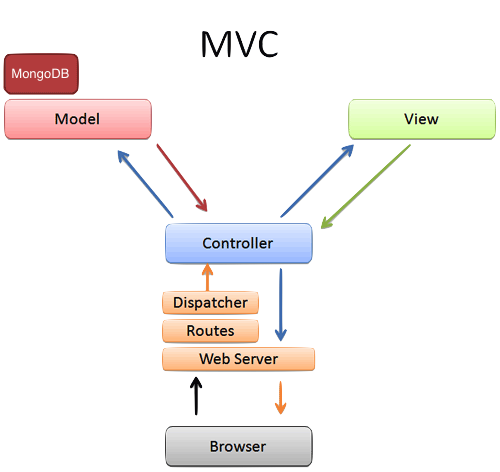
\includegraphics[width=\linewidth]{mvc-architecture-mongo}
     \caption{Patrón de diseño Modelo Vista Controlador (MVC)}\label{Fig:mvc}
   \end{minipage}
\end{figure}

	\begin{figure}[!htb]\centering
	   \begin {minipage}{1\textwidth}
	     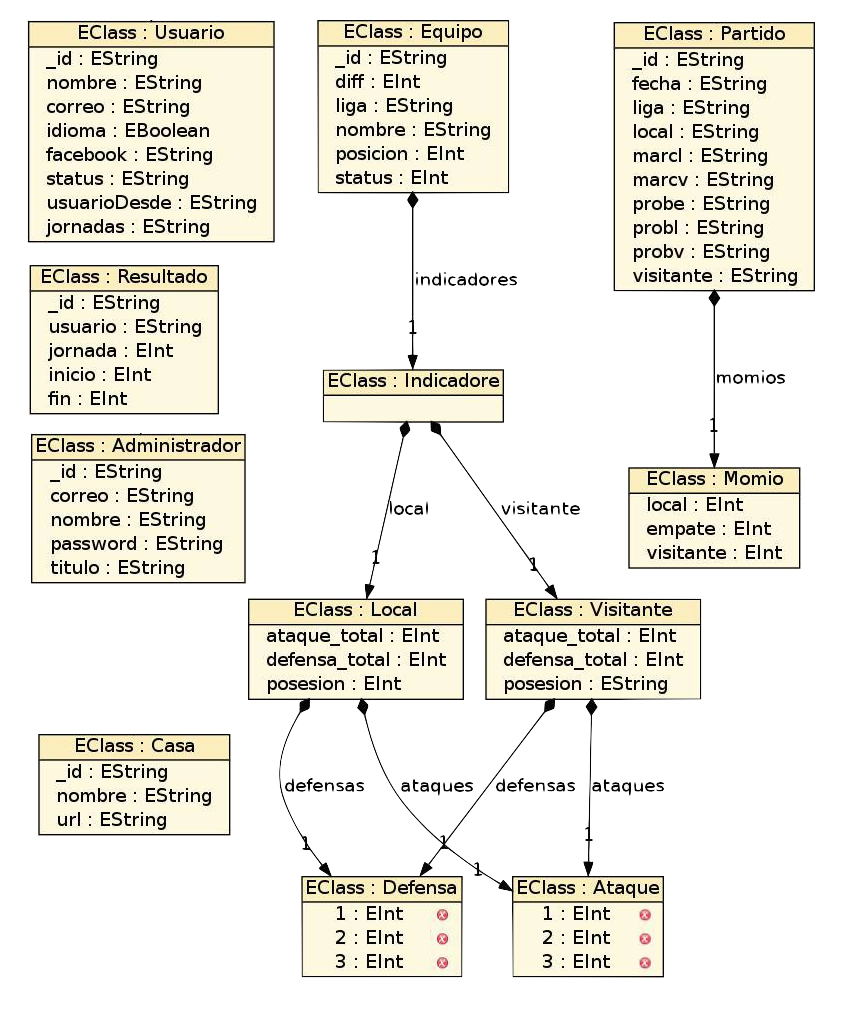
\includegraphics[width=\linewidth]{mongoDB/schema/bd-egobets}
	     \caption{Representación UML de las colecciones de la base de datos de Egobets}\label{Fig:db-egobets}
	   \end{minipage}
	\end{figure}

CodeIgniter es un framework\footnote{Es una estructura de software compuesta de componentes personalizables e intercambiables para el desarrollo de una aplicación. En otras palabras, un framework se puede considerar como una aplicación genérica incompleta y configurable a la que se le puede añadir las últimas piezas para construir una aplicación concreta \cite{upton2007codeigniter}.} de PHP que ahorra tiempo de programación, robustece cualquier sistema y permite al programador alcanzar un grado mayor de sofisticación en su código.

	De su página Web \cite{codeigniterWeb} se pueden destacar las siguientes propiedades:
	\begin{itemize}
		\item Tamaño pequeño. CodeIgniter 2.2 tiene una descarga 2.2MB, incluyendo la guía del usuario.
		\item Documentación clara. La guía que se incluye cuenta con guía y tutoriales para empezar a trabajar de manera muy práctica.
		\item Compatibilidad con casi cualquier servicio de alojamiento. Sólo necesita PHP 5.1.6 y tiene soporte con las bases de datos más comunes incluido MySQL.

		\item Casi no necesita configuración. Todas las variables y opciones de configuración vienen predefinidas a los estándares convenidos en internet.

	\end{itemize}


	Por la naturaleza de la arquitectura MVC es necesario conocer la definición de la estructura de datos para después poder describir en mayor detalle los elementos del sistema. Ahora, hay que recordar que Egobets no utiliza una base de datos relacional por lo que se presenta un diagrama de clases para representar las colecciones que se tienen en la base de datos de Mongo DB.
	\textbf{Definición de la base de datos}
	La base de datos cuenta con seis colecciones principales (Véase la figura~\ref{Fig:db-egobets}):

	\begin{itemize}
		\item Usuario. Se trata de los usuarios que se enrolan al sistema y utilizan los servicios de portal, como las asesorías de apuestas o las predicciones de los partidos.
		\item Administrador. Estos usuarios son los que tienen privilegios para ingresar al portal administrador y gestionar la información del sistema.
		\item Equipo. En esta colección se almacenan todos los equipos de las cinco ligas junto con la posición en la que se encuentra  y la fortaleza con la que cuenta en ese momento.
		\item Partido. Se guardan los partidos de las cinco ligas junto con los marcadores estimados y después los reales. De igual manera se tienen los momios de las casas de apuestas para ese partido.
		\item Casa. En esta colección se almacenan los datos de las casas de apuestas de las cuales se recuperan sus momios para hacer los cálculos de las asesorías de apuestas.
		\item Resultado. Aquí se guarda la cantidad de dinero que obtiene o pierde un usuario en cada jornada.
	\end{itemize}
	Como se puede observar, hay conexiones entre algunas clases. Esto se debe a que las colecciones que tiene MongoDB permiten objetos complejos, de tal manera que un objeto puede contener un arreglo de otros objetos. Para ver un ejemplo de los datos almacenados en la base de datos véase el Apéndice \ref{chap:dbs}.

	Con base en la estructura de datos definida, retómese el patrón de diseño MVC, la propiedad más interesantes de CodeIgniter. Este patrón fue descrito por el noruego Trygve Reenskaug en 1979, y facilita la descripción del sistema de Egobets de una manera más organizada \cite{upton2007codeigniter} \cite{alfredo2005ingenieria}. En los siguientes apartado se describirán  los componentes de Egobets en estas tres dimensiones.


		 \subsection{Modelos}

		La información representa el dominio del problema y la base de datos se abstrae como un conjunto de objetos sobre los cuales recaen todas la acciones. En el modelo, los objetos básico definidos, reflejan las colecciones de la base de datos y a través del conector de base de datos, el modelo modifica los documentos en la base de datos conforme sea requerido.
		En particular, ya se dijo que los datos del sistema de Egobets son los definidos en la figura~\ref{Fig:db-egobets} y la definición de los objetos se pueden ver en el Apéndice~\ref{chap:dbs}. Ahora, recordando que PHP no es un lenguaje cuyos paradigma (inicial) se orientara objetos\footnote{PHP es un lenguaje que soporta objetos, y en particular PHP5 integra más este paradigma, pero no es un lenguaje orientado a objetos. Por ejemplo, muchas de sus funciones principales no pertenecen a ningún objeto.}, los datos que tiene definidos en el modelo son completamente dependientes de la estructura de la base de datos, entonces los objetos utilizados por los modelos son exactamente los mismos definidos en la BD y extraídos con las consultas.

		Como lo menciona Upton en su libro \cite{upton2007codeigniter}, la parte más fundamental es el escribir operaciones ``ABCD''. Es necesario poder Agregar, Borrar, Cambiar y Desplegar la información de las colecciones de la bases de datos. Estas funciones, aunque conceptualmente fáciles de entender, son bastante complejas y escribirlas puede consumir mucho tiempo; sin embargo, son la base de un modelo bien definido, fácil de mantener y reutilizable.

		En concreto, para el portal público de Egobets las siguientes son las funciones utilizadas en los modelos:
		\begin{itemize}
			\item \emph{Usuarios}
				\begin{itemize}
					\item Agregar - A través del modelo, se permite crear un nuevo \emph{usuario} de la plataforma.
					\item Cambiar - Se pueden cambiar los detalles del perfil de un \emph{usuario}, así como las casas de apuestas a las que está suscrito, también es posible actualizar las jornadas ya pagadas del usuario.
					\item Desplegar - Se pueden obtener todos los datos de un usuario en función de su identificador o buscar algún texto en su perfil. También se pueden mostrar los amigos que tiene en Facebook \cite{facebookDocuWeb} en el sistema y las casas de apuestas a las que está suscrito en Egobets.
				\end{itemize}
			\item \emph{Resultados}
			\begin{itemize}
				\item Agregar - Se recibe la información de la cantidad de dinero ganada o perdida por cada usuario e inserta esta información en la colección de \emph{Resultados}.
				\item Desplegar - Se obtienen los \emph{resultados} de ganancias o pérdidas en función del usuario. También se genera la información base para hacer las gráficas de la evolución de dinero en el tiempo.
			\end{itemize}
			\item \emph{Transacciones}
				\begin{itemize}
					\item Agregar - Se permite iniciar e insertar una nueva \emph{transacción} a la base de datos con un estatus de pendiente de pago.
					\item Cambiar - Se puede cambiar y asignar un estatus de pagada junto con una fecha de pago a una \emph{transacción} a través de este modelo.
					\item Desplegar - Para algún usuario, se pueden obtener todas las \emph{transacciones} realizadas.
				\end{itemize}
			\item \emph{Equipos}
				\begin{itemize}
					\item Desplegar - El modelo  de \emph{Equipos} despliega todos los \emph{equipos} registrados en el sistema y estos pueden ser filtrados directamente por:  nombre, identificador o liga a la que pertenecen. También se despliegan los equipos favoritos por cliente.
				\end{itemize}
			\item \emph{Partidos}
				\begin{itemize}
					\item Desplegar - Se muestran todos los \emph{partidos} registrados en el sistema y se pueden filtrar por: el equipo que juega en ellos, el identificador del partido o la liga a la que pertenecen. También este modelo permite obtener las estrellas de cada partido, estas estrellas denotan la confiabilidad que tiene la predicción del resultado de ese partido.
				\end{itemize}
		\end{itemize}

		\subsection{Vistas}

		\graphicspath{{/Users/brunomedina/Dropbox/Tesis-Egobets/egobets-notas/resources/vistas/}}

		Las vistas reflejan el estado del modelo y corresponden a las interfaces que se le presentan al usuario para el manejo de la información. Por lo general, pueden existir múltiples vistas sobre un mismo modelo, por ejemplo puede existir una vista que despliegue un listado de  partidos por liga y al mismo tiempo existir una vista que muestre una gráfica con la cantidad de goles anotados por los equipos locales a través del tiempo. Estas vistas utilizan los mismos modelos, pero la información que despliega es completamente distinta y tiene fines diferentes.

		También una vista puede implementar varios modelos, es decir, mostrar información compleja compuesta por varios elementos de la base de datos. Un ejemplo sería una vista que presente los datos de un partido junto con las estadísticas generales de cada equipo y una gráfica representativa de la cantidad de dinero gastada por los usuarios en las distintas apuestas del partido.

		Las vistas que se tienen en el sistema se pueden enumerar de la siguiente manera:
		\begin{itemize}
			\item \emph{\textbf{Vistas relativas al perfil del usuario}}

			\begin{figure}[!htb]\centering
			   \begin {minipage}{0.7\textwidth}
			     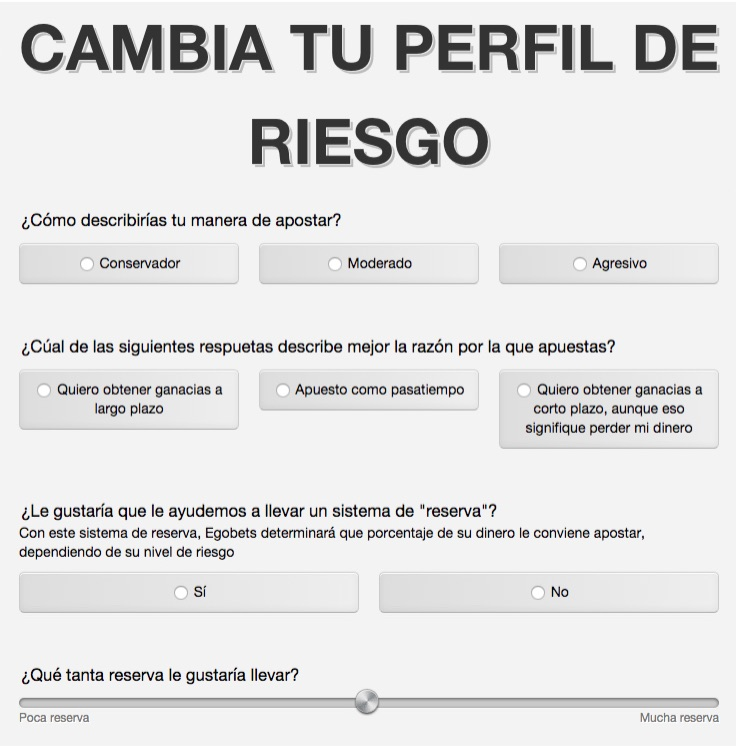
\includegraphics[width=\linewidth]{encuesta}
			     \caption{La encuesta define el perfil de riesgo del usuario}\label{Fig:encuesta}
			   \end{minipage}
			\end{figure}

			En este conjunto de vistas se le permite al usuario gestionar toda la información que tiene que ver con su perfil. Se tienen desde las pantallas para crear una cuenta, hasta las pantallas para editar la encuesta que define las recomendaciones que el usuario recibe.
			A continuación se enlistan estas vistas:
			\begin{itemize}
				\item Sign up. Permite al usuario crear una nueva cuenta para utilizar el sistema (Se puede utilizar Facebook \cite{facebookDocuWeb} para crear el perfil más rápidamente).
				\item Inicio de Sesión. A través de esta pantalla el usuario ingresa sus datos para entrar al sistema.
				\item Restablecer contraseña. Permite al usuario ingresar su correo electrónico para generar una nueva contraseña.
				\item Mi Perfil. En esta vista un usuario puede cambiar sus preferencias como el idioma, si requiere ser notificado cuando haya nuevas recomendaciones y seleccionar las casas de apuestas que utiliza.
				\item Mis Amigos. A través de esta pantalla se pueden ingresar los correos electrónicos de otras personas que tienen cuenta en Egobets para después comparar resultados de sus ganancias.
				\item Encuesta. Como ya se mencionó el riesgo del usuario depende de esta pantalla. El usuario puede ajustarla cada vez que guste cambiar su estrategia de apuesta. Ver imagen~\ref{Fig:encuesta}


			\end{itemize}


			\item \emph{\textbf{Vistas Estáticas}}



			Estas vistas no necesitan ser actualizadas casi nunca, es decir, su contenido es estático. Las páginas estáticas son:
			\begin{itemize}
				\item FAQ. Preguntas frecuentes que ayudan al usuario a comprender más a fondo el sistema (Ver imagen~\ref{Fig:faq}).

				\begin{figure}[!htb]\centering
				   \begin {minipage}{0.75\textwidth}
				     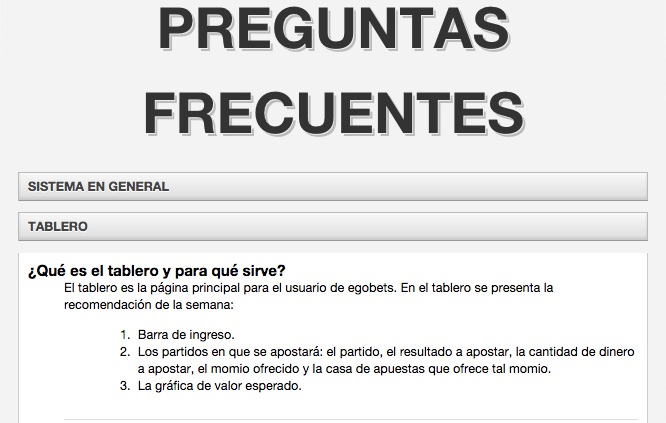
\includegraphics[width=\linewidth]{faq}
				     \caption{La encuesta define el perfil de riesgo del usuario}\label{Fig:faq}
				   \end{minipage}
				\end{figure}

				\item Home Page. La página que recibe a todos los que ingresan al sitio y presenta una bienvenida a los posibles clientes junto con una explicación de lo que es Egobets.com. Además de que contiene el aviso legal.
				\item Términos y condiciones. Presenta el contrato de uso al que se comprometen los clientes al utilizar el sistema.
			\end{itemize}


			\item \emph{\textbf{Vistas relativas a la operación del sistema}}


			En estas vistas se presenta la información de todas las ligas, equipos, partidos y las recomendaciones de apuestas.

			\begin{itemize}

				\item Tablero. La recomendación de apuestas de esta jornada es mostrada al usuario. Se le indica al usuario la cantidad de dinero en porcentaje a apostar en cada una de las apuestas recomendadas y los mejores momios para ese partido por casa de apuestas (Ver figura~\ref{fig:dashboard}).

				\begin{figure}[!htb]\centering
				   \begin {minipage}{0.9\textwidth}
				     \includegraphics[width=\linewidth]{dashboard}
				     \caption{Pantalla de inicio del usuario con recomendaciones de apuestas}\label{fig:dashboard}
				   \end{minipage}
				\end{figure}
				\item Mis Equipos. Una tabla con los equipos preferidos del usuario junto con sus variables de ataque y de defensa.
				\item Tabla de posiciones de la liga. Muestra los nombres de los equipos de la liga seleccionada, variables de ataque y defensa calculadas por el sistema  y el cambio en la tabla de posiciones que han tenido. Se permite al usuario agregar a sus favoritos cualquier equipo para tener un acceso directo a ellos.
				\item Detalle del Equipo. Se presenta el nombre del equipo, su posición en la liga y las estadísticas de ataque y defensa cuando es local o visitante. También se muestran el listado de los partidos próximos que tiene el equipo.
				\item Partidos de la jornada. Consiste en una tabla con los partidos próximos ordenados por fecha del juego. La tabla incluye los equipos participantes, quien es el favorito, el marcador esperado por el sistema y la fecha del juego.
				\item Detalle del partido. Se tienen los equipos que participan, el resultado más probable (junto con su confiabilidad en estrellas), el marcador esperado, la posesión del balón esperada y las estadísticas de ataque y defensa. Estas estadísticas se muestran divididas en las tres categorías. Medio centro, delanteros y definición, para el ataque. Y medio centro, defensas y portero, para la defensa. Cada una de estas variables despliega al ser presionada un histograma con la magnitud esperada de esa variable durante los noventa minutos del partido en intervalos de quince minutos. (Ver imagen~\ref{Fig:partido}).
				\begin{figure}[!htb]\centering
				   \begin {minipage}{0.8\textwidth}
				     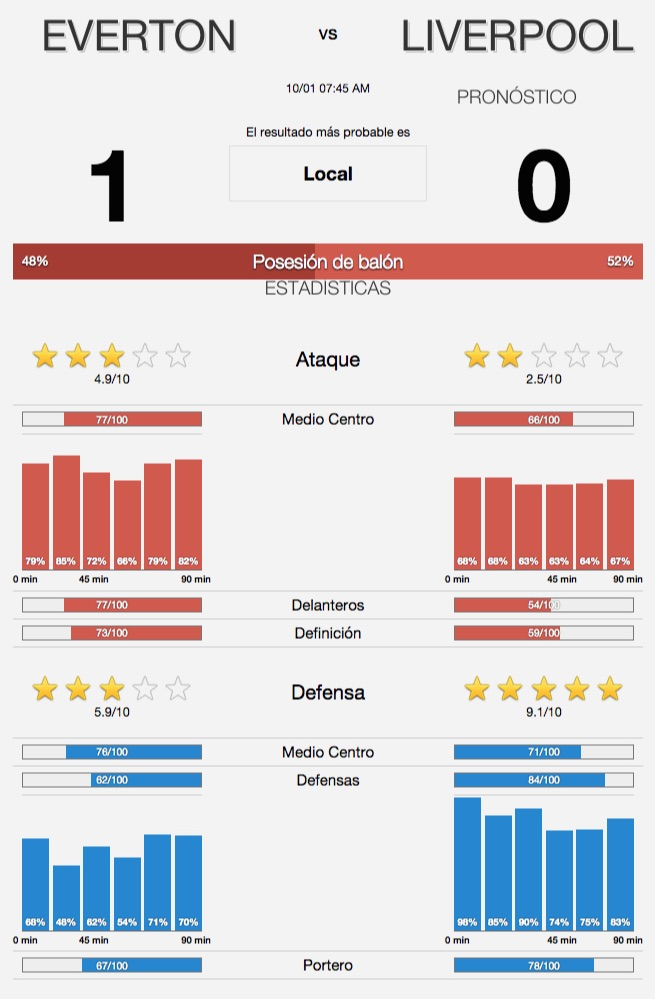
\includegraphics[width=\linewidth]{partido}
				     \caption{Partido con recomendación y estadísticas de los equipos}\label{Fig:partido}
				   \end{minipage}
				\end{figure}

				\item Partidos anteriores. Finalmente esta tabla muestra un comparativo de todos los partidos predichos y su resultado real. Se remarcan los aciertos del sistema y puede ser filtrada por liga.

			\end{itemize}

		\end{itemize}


		Todas la vistas descritas en los párrafos anteriores consisten en archivos HTML5\footnote{HTML viene de HyperText Markup Language, este lenguaje de marcado llegó a la versión 5 utilizada hoy en día el 24 de Octubre del 2014 en el consorcio de la World Wide Web (Básicamente el consorcio de Internet). Para más información leer What is HTML5 de MacLauhlin \cite{mclaughlin2011html5}.} creados dinámicamente en función del código PHP de las vistas. Cada una de estas pantallas cuentan con un archivo CSS\footnote{Cascade Style Sheet, } que aplica el estilo y el diseño al lenguaje de marcado HTML. A su vez, se utiliza Javascript para las animaciones, validaciones y cambios en las propiedades tanto del CSS como del HTML; un ejemplo claro del uso de Javascript es la animación de los gráficos de las estadísticas de los equipos.

		\subsection{Controladores}
		Corresponden a la manipulación de la información a través de sus diversas presentaciones, ofrecen opciones para cambiar el estado del modelo, son los encargados de consultar los modelos y proveer a las vistas los datos dinámicos a mostrar. Básicamente, los controladores implementan el comportamiento o el control de la lógica del sistema, especificando cuándo y como el sistema cambia de estado. Este comportamiento requiere la interacción de múltiples modelos y vistas.
		A continuación se muestra un listado de los controladores del sistema de Egobets junto con las funciones específicas que puede realizar cada uno de ellos.:
		\begin{itemize}
			\item \textbf{Usuario.}
			\begin{itemize}
				\item Restablecer/crear/cambiar un password de una cuenta de usuario.
				\item Calcular el perfil de riesgo del cliente realizando y procesando los resultados de la encuesta.
			\end{itemize}
			\item \textbf{Perfil.} Despliega la información completa del perfil de un usuario,
			\begin{itemize}
				\item Desplegar la información completa del perfil de un usuario junto con los botones necesarios para editarla.
				\item Agregar/quitar una cuenta de Facebook \cite{facebookDocuWeb} al perfil.
				\item Agregar/quitar casas de apuestas al usuario.
 				\item Desplegar información del historial de pagos del usuario.
				\item Agregar/quitar casas de apuestas al usuario.
			\end{itemize}
			\item \textbf{Dashboard.}
			\begin{itemize}
				\item Desplegar la información completa de la recomendación de apuestas de esta jornada al usuario en función de su perfil de riesgo, las casas de apuestas utilizadas y la reserva correspondiente a este usuario.
				\item Agregar la información de las ganancias o pérdidas del usuario en esta semana.
			\end{itemize}
			\item \textbf{Amigos.}
			\begin{itemize}
				\item Desplegar una tabla de posiciones del usuario entre sus amigos respecto a las ganancias de cada uno de ellos. También muestra el listado con la información de sus amigos.
				\item Agregar/quitar amigos de Facebook \cite{facebookDocuWeb} o por correo.
				\item Buscar amigos en el sistema con su correo electrónico.
			\end{itemize}
			\item \textbf{Ayuda.}
			\begin{itemize}
				\item Desplegar la información completa del perfil de un usuario junto con los botones necesarios para editarla.
				\item Agregar/quitar una cuenta de Facebook \cite{facebookDocuWeb} al perfil.
				\item Agregar/quitar casas de apuestas al usuario.
 				\item Desplegar información del historial de pagos del usuario.
				\item Agregar/quitar casas de apuestas al usuario.
			\end{itemize}
			\item \textbf{Sesión.}
			\begin{itemize}
				\item Desplegar la página de inicio de sesión.
				\item Iniciar la sesión del usuario con Facebook o a través de una combinación de correo y password.
				\item Cerrar la sesión de un usuario.
 				\item Crear un nuevo usuario desde cero o con Facebook \cite{facebookDocuWeb} login.
			\end{itemize}
			\item \textbf{Partido.}
			\begin{itemize}
				\item Desplegar la información de los resultados estimados para la jornada en curso.
				\item Desplegar la información de los partidos de la semana pasada con sus respectivos marcadores y las predicciones dadas por el sistema.
			\end{itemize}
			\item \textbf{Equipo.}
			\begin{itemize}
				\item Desplegar la tabla de los equipos favoritos del usuario.
				\item Desplegar las ligas disponibles en el sistema.
				\item Desplegar la tabla de posiciones con todos los equipos que juegan en una liga.
				\item Desplegar la pantalla de detalle de un equipo.
			\end{itemize}
			\item \textbf{Pagos.}
			\begin{itemize}
				\item Desplegar las opciones para comprar jornadas de recomendaciones.
				\item Procesar la transferencia correcta de parte de Paypal de los pagos realizados por el usuario.
			\end{itemize}
			\item \textbf{Ayuda.}
			\begin{itemize}
				\item Desplegar el archivo de preguntas y respuestas de manera correcta.
			\end{itemize}
			\item \textbf{Favoritos.}
			\begin{itemize}
				\item Agregar/Borrar equipos de los favoritos del usuario.
			\end{itemize}

		\end{itemize}

% Todas estas funciones realizadas por los controles definen por completo el sistema de Egobets. Es importante mencionar una función extra que se llama auth(); la cual corre en los constructores de cada uno de los controladores para asegurar que un usuario malintencionado no pueda realizar acciones a nombre de otro. Es decir, que si un usuario cuenta con una combinación válida de nombre de usuario y contraseña, el sistema, por ejemplo, no le permita obtener las ganancias que ha obtenido su peor enemigo en el sistema. De no contar con estas validaciones, se podría construir una llamada HTTP de tal manera que se pudiera obtener esta información.

Todas las funciones listadas en este capítulo conforman en su totalidad el sistema del portal público de egobets.com. Las funciones descritas en el capítulo 3 se ponen a disposición del usuario a través de las interfaces ya definidas y le proporcionan la recomendación de apuestas acorde a su perfil de riesgo. De igual manera, el usuario puede actualizar todos los datos necesarios de su perfil para generar recomendaciones más acorde a sus preferencias.

% En la siguiente sección de este documento, se retoma la función más interesante\footnote{Se considera más interesante una función que muestra recomendaciones de apuestas, que una función que permite al usuario cambiar el idioma del portal. El objetivo de esta tesis es el de mostrar una manera programática de obtener recomendaciones que permitan al usuario apostar de manera estratégica con el fin de obtener ganancias, no el de proveer documentación para la replicación de este sistema a través de ingeniería de software.} del sistema y se explica a mayor detalle su funcionamiento.


% \section{Servicio de asesoría de apuestas}
% \graphicspath{{/Users/brunomedina/Dropbox/Tesis-Egobets/egobets-notas/resources/}}
% \label{sec:service}
%
% En el Capítulo~\ref{chap:mate} se describió el algoritmo detrás de la generación de asesorías de apuestas desde un punto de vista teórico. En este apartado previo a las conclusiones, se hablará de como a través de varias herramientas se logra conseguir la información necesaria para presentarle al usuario una recomendación de apuestas como la de la figura~\ref{fig:dashboard}
%
% 				\begin{figure}[!htb]\centering
% 				   \begin {minipage}{0.9\textwidth}
% 				     \includegraphics[width=\linewidth]{vistas/dashboard}
% 				     \caption{Pantalla de inicio del usuario con recomendaciones de apuestas}\label{fig:dashboard}
% 				   \end{minipage}
% 				\end{figure}
%
% Como ya se mencionó, el algoritmo para generar la asesoría de apuestas se basa en los siguientes pasos:
%  \begin{enumerate}
%  	\item Determinación de apuestas redituables.
%  	\item Selección de apuestas de acuerdo al riesgo del cliente.
%  	\item Cálculo de la proporción del dinero a invertir por apuesta.
%  	\item Determinación del nivel de reservas.
%  	\item Presentar la recomendación.
%  \end{enumerate}
%
% Ahora en términos del sistema estos cinco pasos se llevan a cabo en milisegundos cada vez que el usuario entra a su perfil\footnote{En realidad se genera únicamente si no se tiene la recomendación ya guardada en el cache. Este caché se actualiza cada que hay cambios en los partidos, o cuando el usuario cambia su perfil de riesgo al contestar la encuesta nuevamente.}. Todo este laborioso trabajo que se definió con tanto esfuerzo en el Capítulo~\ref{chap:mate} se ve reducido a una librería de aproximadamente unas quinientas cincuenta líneas de código.
%
% En la sección~\ref{subsec:variables-necesarias} se habla de cuatro variables principales necesarias para poder realizar el algoritmo. Sin embargo, lo que es necesario para poder correr el sistema es: Obtener la información de los partidos, estimar las probabilidades de los partidos y generar las variables de riesgo en función de la encuesta. Estos serán los siguientes apartados del documento.
%
% \begin{figure}[!htb]\centering
%    \begin {minipage}{1\textwidth}
%      \includegraphics[width=\linewidth]{diagramas/sistemas}
%      \caption{Diagrama de herramientas y perfiles}\label{Fig:Sistemas}
%    \end{minipage}
% \end{figure}
%
% \subsection{Información de los partidos y pronósticos}
%
% Se desarrolló un sistema web que recupera al principio de cada temporada todos los partidos que se hayan jugado en las temporadas pasadas, así como el calendario de próximos partidos por jugar. Para lograr la extracción de esta información el sistema cuenta con un ``Web Scraper'' que consigue la información de la página de ESPN y la transforma en objetos que después son persistidos en la base de datos. Finalmente, esta información se organiza en un documento CSV para ser descargado por los administradores.
%
% El proceso que se lleva a cabo en el \emph{Back Office} para alimentar el \emph{Portal público} (Ver la figura~\ref{Fig:flujo}), se puede describir de la siguiente manera:
% \begin{enumerate}
% 	\item A través del \emph{Sistema de recopilación} los administradores descargan de la página de Internet de ESPN los resultados de todos los partidos de la temporada junto con la información de los próximos partidos por jugar  de cada una de las ligas Europeas.
% 	\item Los datos recopilados permiten a los administradores generar un conjunto de archivos de texto con toda la información de los resultados de los últimos partidos y las fechas de los próximos partidos.
% 	\item Los administradores usan estos archivos para alimentar el \emph{Sistema de estimación} y calcular los pronósticos de los próximos partidos y las probabilidades de los resultados.
% 	\item Se obtienen los archivos que contienen la información de los próximos partidos así como la información de los equipos por liga y su desempeño en la temporada en curso.
% 	\item En el \emph{Portal administrativo} se ingestan los archivos obtenidos con la información de los próximos partidos, resultados de partidos anteriores y las estadísticas de los equipos en la temporada en curso.
% 	\item Finalmente, con la nueva información ingresada, los usuarios podrán disfrutar en el \emph{Portal público} sus recomendaciones personalizadas de apuestas.
% \end{enumerate}
%
% \begin{figure}[!htb]\centering
%    \begin {minipage}{1\textwidth}
%      \includegraphics[width=\linewidth]{diagramas/flujo}
%      \caption{Proceso de alimentación del sistema}\label{Fig:flujo}
%    \end{minipage}
% \end{figure}
%
% \subsubsection{Web Scraper}
% El proceso de ``Web Scraping'' consiste en extraer y crear representaciones estructuradas con la información de un sitio Web en particular. HTML, el lenguaje de marcado usado para darle estructura a la información de las páginas web está sujeta a muchos cambios, especialmente cuando se actualiza su estilo. Ya que las técnicas de extracción se basan en el lenguaje de marcado, un solo cambio puede llevar a extraer datos incorrectos o incompletos \cite{cording2011algorithms}.
%
% Las técnicas de ``Web Scraping'' permiten, por ejemplo, que una compañía monitoree los precios de los productos de sus competidores. De igual manera le permiten a Egobets, conseguir la última información detallada con la información de las fechas de los partidos, marcadores, tiros a gol, posesión del balón y nombres de los equipos.
%
% Si el dueño de la información no provee de una API abierta, el remedio (como en el caso de Egobets) es el de escribir un programa que apunte a la información desplegada en la página Web. Las propiedades buscadas en un scraper son:
% \begin{itemize}
% 	\item Ser tan tolerante como pueda ser posible a cambios en el lenguaje de marcado.
% 	\item Ser lo suficientemente rápido como para ofrecer respuestas en milisegundos y evitar ``time-outs'' durante el consumo del servicio.
% 	\item No tener restricciones en los patrones que conforman la estructura del HTML del sitio. En específico esto implica que el servicio debe ser lo suficientemente bueno como para interpretar de la mejor manera la información aún incluso si el HTML se encuentra mal formado
% \end{itemize}
%
% Cording, P. \cite{cording2011algorithms} presenta en su tesis de maestría un estudio de como realizar un scraper que base su funcionamiento en la coincidencia aproximada de los patrones de un árbol, esta es la base de muchas de las librerías que existen (incluyendo la que se usa en este trabajo). Para realizar esta tarea se utiliza una librería de código abierto que permite manipular DOM\footnote{W3schools \cite{domWeb} lo define como: ``Documento W3C Object Model (DOM) es una interfaz de la plataforma y de lenguaje neutro que permite a los programas y scripts acceder y actualizar dinámicamente el contenido, la estructura y el estilo de un documento''. La especificación formal se puede leer en la recomendación \cite{wood1998document}.} de HTML y conseguir la información necesaria, esta libreria se llama: PHP Simple HTML DOM Parser.
%
% \textbf{Un ejemplo de uso}
%
% Supóngase el siguiente HTML:
%
% \lstset{language=HTML}
% \begin{lstlisting}[frame=single]
% <div class="team-names">
% 	<div class="team-name">
% 		<span>
% 			<img src="http://espncdn.com/teamlogos/soccer/500/102.png" alt="Villarreal" width="22">
% 			Villarreal
% 		</span>
% 	</div>
% 	<div class="team-name">
% 		<span>
% 			<img src="http://espncdn.com/teamlogos/soccer/500/93.png" alt="Athletic Bilbao" width="22">
% 			Athletic Bilbao
% 		</span>
% 	</div>
% </div>
% \end{lstlisting}
%
% Ahora analícese el siguiente código:
%
% \lstset{language=PHP}
% \begin{lstlisting}[frame=single]
% 	$aux = $table->find('.team-name',0);
% 	$nomEquipoLocal = $aux;
% 	$partido['prints']['local_nom']= $nomEquipoLocal;
% 	$idEspnEquipoLocal = trim(strstr(substr(strstr($aux->innertext, 'soccer/500/'), strlen('soccer/500/')),'.png',true));
% \end{lstlisting}
%
%
% Con este código se pueden obtener los nombres del equipo local y el identificador que le asigna ESPN a sus equipos. Esto es gracias a que \emph{``find('.team-name',0)''} recorre todo el árbol DOM y encuentra todas las ocurrencias de la clase con nombre \emph{``team-name''} el cero que se le proporciona a la función \emph{find} regresa el primer elemento encontrado. De ahí, la propiedad \emph{``->innertext''} muestra la cadena de caracteres plana que contiene ese elemento, por lo que basta con hacer un manejo de cadenas de caracteres para obtener el identificador del equipo que se nombra el archivo PNG del logo del equipo. Para más ejemplos y documentación de como utilizar la librería dirigirse a \cite{sourceparserWeb}.
%
%
% % \end{enumerate}
%
% \subsection{Generar las variables en función de la encuesta}




%
% \begin{enumerate}
% 	\item \emph{Recomendación personalizada de apuestas en fútbol:} Cada persona es diferente y debe ser tratada de forma única, en Egobets se determina el perfil de riesgo de cada usuario mediante una encuesta y se le recomienda apuestas a su medida, de tal forma que pueda obtener ganancias y sentirse cómodo al mismo tiempo.
% 	\item \emph{Pronósticos:} Para cada partido se proporcionan, entre otros: marcador final más probable, resultado más probable y el nivel de posesión de balón de cada equipo.
% 	\item \emph{Estadísticas:} A través de éstas se pueden analizar las fortalezas y debilidades de los equipos favoritos del usuario.
% \end{enumerate}
%
% \subsection{Encuesta}
% \label{subsec:encuesta}
%
%
% \textbf{Perfil de riesgo}
%
%
% El perfil de riesgo sirve para poder personalizar la asesoría de apuestas y se calcula a través de las respuestas proporcionadas en la encuesta de perfil de riesgo.
%
% De forma genérica hay tres perfiles de riesgo:
% \begin{enumerate}
% 	\item Agresivo: Toma riesgos altos para poder obtener la mayor cantidad de ganancias posibles en el corto plazo.
% 	\item Conservador: Apuesta a lo más seguro para proteger su dinero lo más posible, busca ganancias al largo plazo.
% 	\item Moderado: Término medio entre agresivo y conservador.
% \end{enumerate}
%
% \textbf{Sistema de reservas}
%
% En \emph{Egobets.com} se entiende que cada persona es diferente, que cada apuesta es diferente y debe ser analizada de forma individual, por eso se ha desarrollado el sistema de reservas que determina cuánto dinero apostar en la recomendación de la semana.
%
% La reserva es la cantidad de dinero que no se apostará, sirve para poder seguir apostando en semanas posteriores en el caso en que se lleguen a tener pérdidas.
%
%
% Se toman en cuenta tres factores: la volatilidad de la apuesta, la ganancia esperada de ésta y el nivel de riesgo deseado del cliente. Se combina esta información en un modelo probabilístico que proporciona la cantidad a apostar. Mediante este sistema se busca de proteger al cliente de pérdidas potenciales.
%
% Beneficios:
% \begin{enumerate}
%
% 	\item Protege su dinero de pérdidas potenciales.
% 	\item Permite recuperarse con mayor velocidad de semanas con pérdidas.
% 	\item Permite dar una estructura de fondo de inversión a las apuestas al obtener un sistema de interés compuesto.
%
% \end{enumerate}
%
% Costos:
% \begin{enumerate}
% 	\item Se restringe la cantidad de ganancias a corto plazo.
% \end{enumerate}
%
% Es un sistema a largo plazo, no se recomienda a personas que desean incurrir en riesgos elevados en beneficio de la posibilidad de obtener mayores ganancias.
%
%
% \subsection{Tablero de apuestas}
%
% El tablero es la página principal para el usuario de \emph{Egobets.com}. En el tablero se presenta la recomendación de la semana:
% \begin{enumerate}
%
% \item Barra de ingreso.
% \item Los partidos en que se apostará: el partido, el resultado a apostar, la cantidad de dinero a apostar, el momio ofrecido y la casa de apuestas que ofrece tal momio.
% \item La gráfica de valor esperado.
% \end{enumerate}
%
% En \emph{Egobets.com} se le da seguimiento a cada uno de nuestros clientes. Con esta información se puede monitorear la evolución del ingreso y así dar las recomendaciones de acuerdo al nivel de ganancias o pérdidas. Es importante que esta información sea verdadera para poder brindar el mejor servicio posible.
% \begin{enumerate}
%
% 	\item \textbf{¿Se pueden hacer recomendaciones de resultados que no sean los más probables?}
% \end{enumerate}
%
%
% Sí, depende del perfil de riesgo y de lo que pague la casa de apuestas en tal partido. En algunas ocasiones es recomendable apostar en contra del favorito si el pago es suficientemente grande. Si se tiene activado el sistema en contra de favoritos (en el menú perfil) o si el perfil es muy agresivo se presentarán muchas recomendaciones de este tipo.
%
% La gráfica de valor esperado es una herramienta visual que permite ver cuáles son los posibles resultados de la recomendación de la semana. En \emph{Egobets.com} se conoce que todas las apuestas tienen un riesgo y mediante esta gráfica se puede cuantificar: Cada barra representa la probabilidad de que se gane o pierda la cantidad indicada debajo de ella, mientras más grande sea la barra mayores probabilidades hay de que tal resultado ocurra.
%
%
%
% \subsection{Pronósticos}
% Pronósticos: Se pronostica el marcador final, la posesión del balón y el ganador del encuentro. Al poner el apuntador sobre el resultado más probable aparece el grado de confiabilidad del pronóstico.
%
%
% En \emph{Egobets.com} se presentan los equipos mediante un power ranking. Con base en las estadísticas de los partidos y dados sus resultados, se pronostica cuál será la tabla de posiciones al finalizar dicha liga.
%
%
% \subsection{Estadísticas}
%
%
% En orden de aparición: Una estrella indicando si el equipo está o no marcado como uno de los favoritos, la posición en el power ranking, el nombre del equipo, el índice de ataque general del equipo, el índice de defensa general del equipo y por último el cambio dentro de la tabla de power ranking.
%
% \begin{enumerate}
%
% \item Índice de ataque general: Con calificación de una a cinco estrellas o de uno a diez (abajo). Representa la capacidad general del equipo para atacar.
% \item Índices de medio centro, delanteros y definición: Con una calificación de cero a cien. Representan la capacidad de controlar el medio centro, de atacar a portería y de precisión de los tiros, respectivamente.
% \item Índice de defensa general: Con calificación de una a cinco estrellas o de uno a diez (abajo). Representa la capacidad general del equipo para defender.
% \item Índices de medio centro, defensas y portero: Con una calificación del cero a cien. Representan la capacidad de defender en el centro, de los defensas y del portero, respectivamente.
% \item Al hacer click en las variables mencionadas en 2 o 4 se tienen acceso a la evolución de tales variables desde el minuto 0 hasta el 90 de un partido.
% \end{enumerate}
%
% \begin{enumerate}
%
% 	\item \emph{Resultados de la jornada anterior:} Se presenta el partido, el marcador real, el marcador pronosticado y el resultado pronosticado. Esto con el fin de que los usuarios puedan comparar lo pronosticado y lo que en verdad ocurrió.
% 	\item \emph{Pronósticos de la jornada actual:} Se presenta el partido, el resultado pronosticado (o favorito), el marcador pronosticado y la fecha del encuentro. Además al poner el apuntador encima de un partido se presenta el grado de confiabilidad del pronóstico.
% \end{enumerate}
%
% Además para cada tabla se pueden presentar los resultados de una liga en particular al seleccionarla en el recuadro de arriba.
%
% \section{Alimentando el sistema}
% \label{sec:inserting-data}
%
% \begin{figure}[!htb]\centering
%    \begin {minipage}{1\textwidth}
%      \includegraphics[width=\linewidth]{sistemas}
%      \caption{Diagrama de sistemas y usuarios}\label{Fig:Sistemas}
%    \end{minipage}
% \end{figure}
%
% \begin{figure}[!htb]\centering
%    \begin {minipage}{1\textwidth}
%      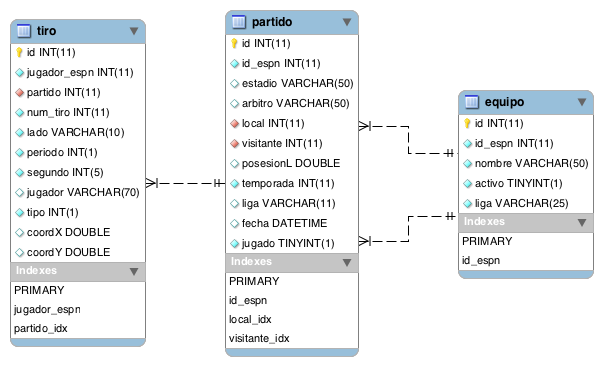
\includegraphics[width=\linewidth]{erd-pronosticos}
%      \caption{Diagrama de entidad-relación de la BD del recopilador}\label{Fig:erd-pronosticos}
%    \end{minipage}
% \end{figure}
%
% El proceso que se lleva a cabo en el \emph{Back Office} para alimentar el \emph{Portal público} (Ver la figura~\ref{Fig:flujo}), se puede describir de la siguiente manera:
% \begin{enumerate}
% 	\item A través del \emph{Sistema de recopilación} los administradores descargan de la página de Internet de ESPN los resultados de todos los partidos de la temporada junto con la información de los próximos partidos por jugar  de cada una de las ligas Europeas.
% 	\item Los datos recopilados permiten a los administradores generar un conjunto de archivos de texto con toda la información de los resultados de los últimos partidos y las fechas de los próximos partidos.
% 	\item Los administradores usan estos archivos para alimentar el \emph{Sistema de estimación} y calcular los pronósticos de los próximos partidos y las probabilidades de los resultados.
% 	\item Se obtienen los archivos que contienen la información de los próximos partidos así como la información de los equipos por liga y su desempeño en la temporada en curso.
% 	\item En el \emph{Portal administrativo} se ingestan los archivos obtenidos con la información de los próximos partidos, resultados de partidos anteriores y las estadísticas de los equipos en la temporada en curso.
% 	\item Finalmente, con la nueva información ingresada, los usuarios podrán disfrutar en el \emph{Portal público} sus recomendaciones personalizadas de apuestas.
%
% \begin{figure}[!htb]\centering
%    \begin {minipage}{1\textwidth}
%      \includegraphics[width=\linewidth]{flujo}
%      \caption{Proceso de alimentación del sistema}\label{Fig:flujo}
%    \end{minipage}
% \end{figure}
% \end{enumerate}
%
%


% \section{Descripción General}
% \label{sec:description}
%
% El ecosistema de Egobets consiste principalmente de cuatro piezas de software. Ver la figura~\ref{Fig:Sistemas}.
%
%
%
%
% \begin{figure}[!htb]\centering
%    \begin {minipage}{1\textwidth}
%      \includegraphics[width=\linewidth]{sistemas}
%      \caption{Diagrama de sistemas y usuarios}\label{Fig:Sistemas}
%    \end{minipage}
% \end{figure}
%
% El Sistema de recopilación de información y estadísiticas de los partidos (\emph{Sistema de recopilación}), el \emph{Portal administrativo} y el \emph{Portal público} corren bajo una arquitectura cliente servidor en la nube de Amazon Web Services; mientras que el Sistema de estimación de probabilidades (\emph{Sistema de estimación}) corre en un ordenador personal.
%
%

%
% \subsection{Piezas de software y su interacción}
%
% \begin{figure}[!htb]\centering
%    \begin {minipage}{1\textwidth}
%      \includegraphics[width=\linewidth]{flujo}
%      \caption{Diagrama de flujo de información}\label{Fig:flujo}
%    \end{minipage}
% \end{figure}
%
% El proceso que se lleva a cabo en el \emph{Back Office} para alimentar el \emph{Portal público} (Ver la figura~\ref{Fig:flujo}), se puede describir de la siguiente manera:
% \begin{enumerate}
% 	\item A través del \emph{Sistema de recopilación} los administradores descargan de la página de Internet de ESPN los resultados de todos los partidos de la temporada junto con la información de los próximos partidos por jugar  de cada una de las ligas Europeas.
% 	\item Los datos recopilados permiten a los administradores generar un conjunto de archivos de texto con toda la información de los resultados de los últimos partidos y las fechas de los próximos partidos.
% 	\item Los administradores usan estos archivos para alimentar el \emph{Sistema de estimación} y calcular los pronósticos de los próximos partidos y las probabilidades de los resultados.
% 	\item Se obtienen los archivos que contienen la información de los próximos partidos así como la información de los equipos por liga y su desempeño en la temporada en curso.
% 	\item En el \emph{Portal administrativo} se ingestan los archivos obtenidos con la información de los próximos partidos, resultados de partidos anteriores y las estadísticas de los equipos en la temporada en curso.
% 	\item Finalmente, con la nueva información ingresada, los usuarios podrán disfrutar en el \emph{Portal público} sus recomendaciones peronalizadas de apuestas.
% \end{enumerate}
%
%
% \subsection{Sistema de recopilación de información y estadísticas de los partidos}
% \graphicspath{{/Users/brunomedina/Dropbox/Tesis-Egobets/egobets-notas/resources/recopilador/}}
%
%
% \subsubsection{Tecnologías destacadas}
%
% \begin{itemize}
% 	\item \textbf{Servidor LAMP.} Esta es una de las configuraciones más populares para servidores web.
% 		Una de las principales ventajas de utilizar una arquitectura LAMP es que la mayoría del software utilizado corre bajo la ``Licencia Pública General de GNU'', esta licencia de uso permite a los programadores que utilizan este software, ser capaces de ver el código fuente y en muchos casos le permiten modificarlo y compartirlo \cite{lozano2008software}.
% 	El famoso acrónimo representa lo siguiente :
% 	\begin{itemize}
% 		\item Apache. El servidor HTTP, encargado de recibir y procesar las llamadas HTTP, nació hace diecisiete años como un proyecto por desarrollar un software robusto, de grado comercial, modular y gratuito para servir peticiones (Web) HTTP. Algunas de las ventajas con las que cuenta son \cite{apacheWeb}:
% 		\begin{itemize}
% 			\item Gran variedad de módulos. Existen muchos módulos que la comunidad desarrolla para atacar las problemáticas diarias, gracias a que su comunidad es muy activa estos desarrollos nunca acaban.
% 			\item Fácil de administrar. El soporte de la comunidad y su extensivo uso permite que sea muy sencillo encontrar documentación de como realizar las funciones básicas de administración de servidores como la creación de nuevos dominios, implantación de certificados SSL, etc.
% 			\item No importa el sistema operativo, Apache corre en UNIX, Windows, Mac y en la gran mayoría de sistemas operativos.
% 			\item Corre bajo la licencia pública general de GNU.
% 		\end{itemize}
%
% 		\item MySQL. Base de datos relacional que permite al sistema persistir toda la información recuperada del internet. Las principales características de MySQL son \cite{mysqlWeb}:
% 		\begin{itemize}
% 			\item Sistema de administración. El servidor MySQL provee las herramientas para agregar, ingresear, procesar y desplegar la información guardada en la base de datos.
% 			\item Las bases de datos MySQL son relacionales. La información se guarda en tablas separadas en vez de poner todo junto en un solo lugar. Las estructuras de base de datos están organizadas en archivos físicos optimizados para la velcidad. El modelo lógico con objetos como bases de datos, tablas, vistas, tuplas y columnas ofrece un ambiente de programación flexible. Y MySQL se asegura de que se respeten los tipos de relaciones entre tablas como puede ser uno a uno, uno a varios, únicas, u opcionales. Una base de datos bien diseñada nunca permitirá información incosistente, duplicada, huerfana, fuera de fecha o perdida.
% 			\item Corre bajo la licencia Pública General de GNU. Por lo que se puede modificar y ser utilizado por cualquiera.
% 		\end{itemize}
% 				\item PHP:
%
%
% 	\item Code Igniter. Es un framework\footnote{Es una estructura de software compuesta de componentes personalizables e intercambiables para el desarrollo de una aplicación. En otras palabras, un framework se puede considerar como
% una aplicación genérica incompleta y configurable a la que se le puede añadir las últimas piezas para construir una aplicación concreta.} de PHP que ahorra tiempo en le programación, robustece tu sistema y permite al programador alcanzar un grado mayor de sofisticación en su código. Uno de los puntos interesantes de este framework es que utiliza el patrón de diseño conocido como Modelo Vista Controlador (MVC), este patrón fue descrito por el noruego Trygve Reenskaug en 1979.
% 	Sobre el libro de Upton \cite{upton2007codeigniter} se tiene una aproximación a este patrón de diseño en CodeIgniter:
% 	\begin{itemize}
% 		\item Modelos, son objetos que representan los datos. Estos objetos reflejan las tabla de la base de datos y pueden modificarla conforme sea requerido. Los modelos también realizan operacioens a los datos según sea necesario.
% 		\item Vistas, reflejan el estado del modelo. Son las responsables de desplegar la información al usuario final. En este caso específico, todas las vistas son representaciones HTML del contenido.
% 		\item Controladores, ofrecen opciones para cambiar el estado del modelo. Son los encargados de consultar los modelos. Proveen a las vistas los datos dinámicos a mostrar.
% 	\end{itemize}
% 	De su página Web \cite{codeigniterWeb} se pueden destacar las siguientes propiedades:
% 	\begin{itemize}
% 		\item Tamaño pequeño. CodeIgniter 2.2 tiene una descarga 2.2MB, incluyendo la guía del usuario.
% 		\item Documentación clara. La guía que se incluye cuenta con guía y tutoriales para empezar a trabajar de manera muy práctica.
% 		\item Compatibildad con casi cualquier servicio de alojamiento. Sólo necesita PHP 5.1.6 y tiene soporte con las bases de datos más comunes incluído MySQL.
%
% 		\item Casi no necesita configuración. Todas las variables y opciones de configuración vienen predefinidas a los estandares convenidos en internet.
%
% 	\end{itemize}
%
%
% 	\item PHP Simple HTML DOM Parser
% 	Es un script de PHP que permite interpretar el HTML DOM de una página web y permite manipularlo de manera muy sencilla. Requiere PHP 5 o mayor, soporta archivos HTML mal formados y permite encontrar las etiquetas HTML con selectores como lo haría jQuery. Con una simple línea de código basta para extraer los contenidos de una página HTML \cite{htmlparserWeb}.
% 	\cite{chen2009php} \cite{chowdhury2014intelwiki}
% 	\item Bootstrap. Es un framework elegante, intuitivo y poderoso que agiliza y facilita el desarrollo Web de front-end Su principal objetivo es facilitar el desarrollo de sitios móviles y responsive.
% 	Documentación amplia y detallada, docenas de elementos HTML, componentes CSS e increíbles plugins de jQuery son algunas de sus principales características\cite{bootstrapWeb}.
% 	\cite{otto2010bootstrap}
% 	\cite{cochran2012twitter}
%
% \end{itemize}
%

% % Definir lo que es un scraper
% %
% %
% % Definir las páginas que se buscan y como se recorren
% %
% % Definir los objetos finales de la base de datos que se consumen.
% %
% %
%
%
% \subsubsection{Descripción de su funcionamiento}
%
% \begin{enumerate}
% 	\item \textbf{Equipos de la temporada.}
% 	Para poder comenzar la recuperación de información, es importante contar con los equipos que estén jugando esta temporada. Dependiendo de los resultados de la temporada anterior, los equipos que hayan quedado hasta abajo en la tabla de posición descienden a ligas menores y a su vez suben los mejores de estas ligas. Ver figura~\ref{Fig:los-equipos}
% 	\begin{figure}[!htb]\centering
% 	   \begin {minipage}{1\textwidth}
% 	     \frame{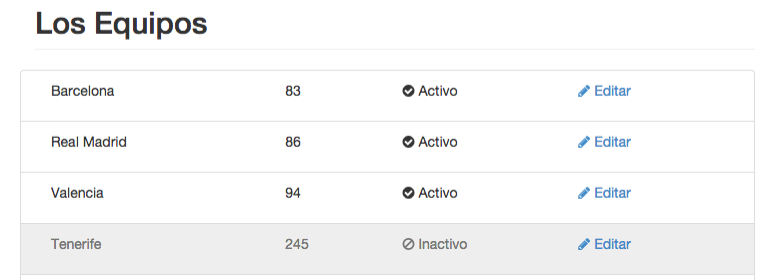
\includegraphics[width=\linewidth]{los-equipos}}
% 	     \caption[Ejemplo de equipos de la liga española]{Ejemplo de equipos de la liga española\footnotemark }\label{Fig:los-equipos}
% 	   \end{minipage}
% 	\end{figure}
%
%
% 	\item \textbf{Calendario de próximos partidos.}
% 	\begin{figure}[!htb]\centering
% 	   \begin {minipage}{1\textwidth}
% 	     \frame{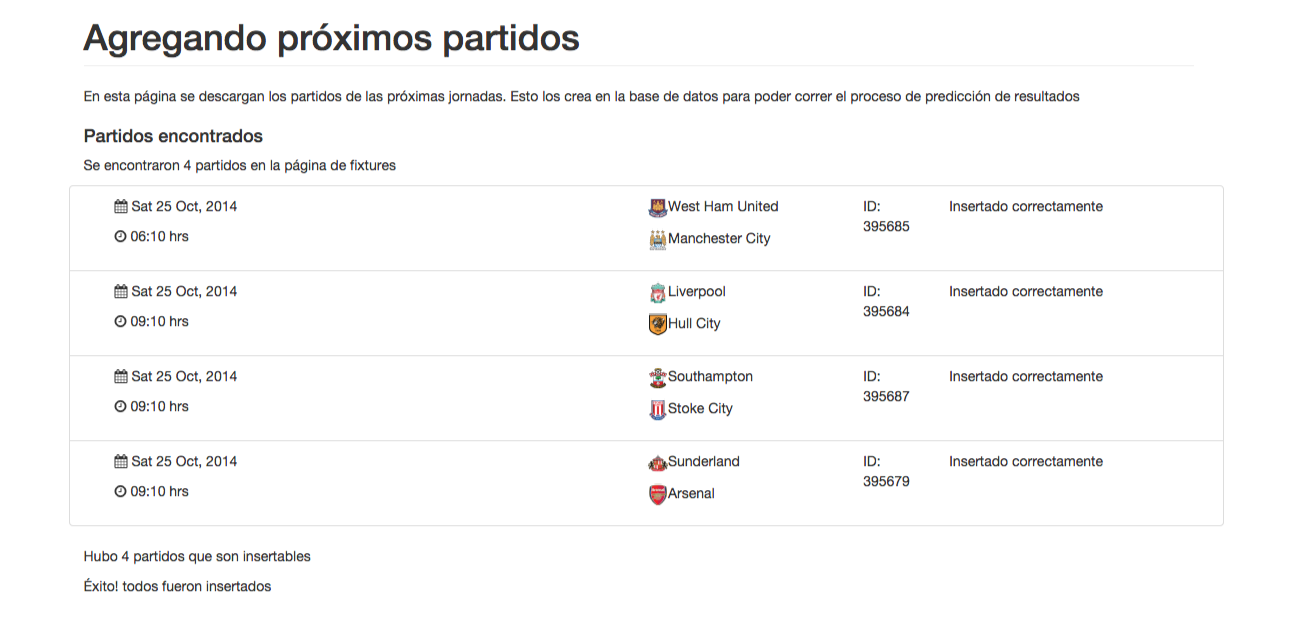
\includegraphics[width=\linewidth]{proximos-partidos}}
% 	     \caption{Recuperación de próximos partidos}\label{Fig:proximos-partidos}
% 	   \end{minipage}
% 	\end{figure}
%
% 	\item \textbf{Estadísticas e información de partidos jugados.}
% 	\begin{figure}[!htb]\centering
% 	   \begin {minipage}{1\textwidth}
% 	     \frame{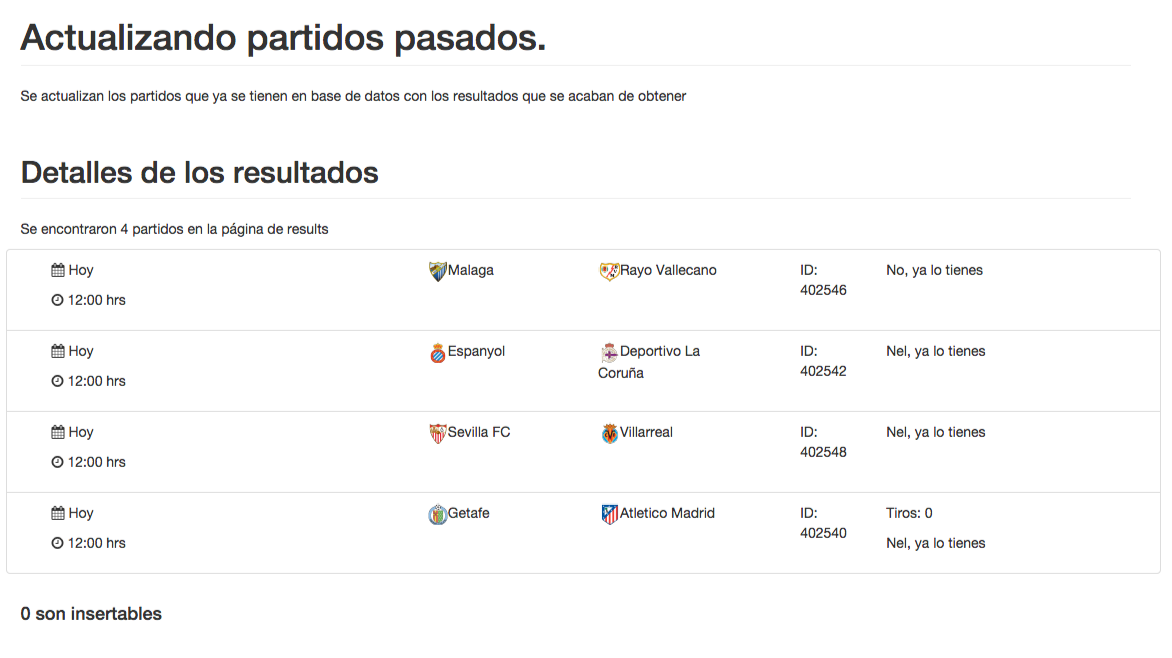
\includegraphics[width=\linewidth]{pasados-partidos}}
% 	     \caption{Recuperación de resultados de partidos ya jugados}\label{Fig:pasados-partidos}
% 	   \end{minipage}
% 	\end{figure}
% 	\item \textbf{Generación de archivos con resultados.}
% 	Es importante mencionar que se usan aproximadamente los últimos quinientos partidos para la generación de los archivos, esto implica que se deben tener en base de datos los equipos que participaron en las pasadas dos temporadas de juegos. Por este motivo de pueden encontrar equipos que se encuentran en el sistema con la bandera de inactivos.
%
% \end{enumerate}
%
%
%
%
%
%
%
%
%
%
%
%
%
% \subsection{Sistema de estimación de probabilidades}
% Adicionalmente en esta sección se describirá el funcionamiento del Sistema de Estimación. Sin embargo, al ser un conjunto de programas en \emph{Fortran} que son ajenos al autor, no se profundizará en los detalles del desarrollo del mismo. Sin embargo, se dará la pauta para entender como se podrían generar probabilidades y pronósticos de los partidos.
%
% \subsubsection{Predicciones}
%
%
%
% \cite{rue2000prediction}
%
% \cite{baio2010bayesian}
%
% \cite{dixon2004value}
%
% \cite{koopman2013dynamic}
%
%  \subsubsection{Tecnologías destacadas}
%
% \begin{itemize}
% 	\item \textbf{Fortran}
% 	\cite{robison1996c++}
% 	\cite{veldhuizen1997will}
% \end{itemize}
%
% \subsubsection{Descripción de su funcionamiento}
%
% Montecarlo
% Poisson
% Nonormal
% Markov
%
%
% \subsection{Portal administrativo}
%
% \subsubsection{Sitio web para los administradores}
%
%  \cite{alfredo2005ingenieria}
%
%  \subsubsection{Tecnologías destacadas}
%
%  \begin{itemize}
%  	\item LNNP
%  	\item Code Igniter
%  	\item Raphael
%  \end{itemize}
%
%  \subsubsection{Diagrama de base de datos}
%
%  \subsubsection{Descripciónde su funcionamiento}
%
%  \begin{itemize}
%  	\item CRUD
%  	\item Ingesta de archivos
%
%  \end{itemize}
%
%
% \section{Portal público Egobets.com}
%
% \subsection{Características principales}
% \subsubsection{Sitio web para los jugadores}
% \subsubsection{Tecnologías destacadas}
%
%  \begin{itemize}
%  	\item LNNP
%  	\item Code Igniter
%  	\item Parallax
%  \end{itemize}
%
% \subsubsection{Módulos}
%
%  \begin{itemize}
%  	\item Tablero
%  	\item Mis Equipos
%  	\item Ligas
%  	\item Partidos
%  	\item Perfil
%  	\item Pagos
%  	\item Perfil de riesgo
%  	\item Sistemas de reserva
%  \end{itemize}
%
%
%
